\chapter{Ramping parameter under the random graph model} % (fold)
\label{cha:ramping_parameter_under_the_random_graph_model}

Previous work~\cite{Sindel:2009vd} provided a connection between the clustered structure of a graph and an interpretation of concentration risk.
The methodology presented by the authors considered the effects of removing edges with weight under given a varying threshold on the community structure of a fully connected obligor-correlation matrix.
In particular, by computing the variation of the component structure of the graph, the authors have shown how to analyse concrete credit portfolios and identify sets of highly connect assets.


This thesis builds upon the aforementioned model and aims at describing the expected behaviour of the ramping parameter model for theoretical graph generation models.
In this chapter, we focus on the random graph model, a well understood theoretical graph model, described in section~\vref{sec:random_graph_model}.

In particular, it tries to describe the expected behaviour of the curve designed by the~\cite{Sindel:2009vd} the problem from the perspective of having
large, idealized portfolios 
and a random graph model that generates them.





\section{The ramping parameter model} % (fold)
\label{sec:the_ramping_parameter_model}


The approach proposed by~\cite{Sindel:2009vd} for quantifying the concentration risk of a loan portfolio works can be summarized as follows:
\begin{itemize}
	\item The mutual dependency between the obligors in a portfolio is represented by a matrix $\rho_{ij}$. This matrix is symmetric, the values $\rho_{ij} \in [0,1]$, and it will be called correlation matrix throughout the remainder of this document.
	\item A so-called ramping parameter $\ramp \in [0,1]$ is used to define the effective correlation matrix $\rho_{ij}(\ramp)$ given the value of this  parameter:
	\begin{equation}
	\rho_{ij}(\ramp) = 
		\begin{cases}
		1 \text{ if } \rho_{ij} \ge \ramp,\\
		0 \text{ otherwise}.
		\end{cases}
	\end{equation}
	At $\ramp = 0$, the effective matrix will contain all connections in the original matrix. At $\ramp = 1$, all obligors in the effective matrix will be disconnected.
	
	\item The exposure-dependence is taken into account by computing the “effective” exposure for every value of $\ramp$.
\end{itemize}

To properly account for the Concentration Risk we compute the ratio $R(ρ∗)$ of the maximum of all exposures of all identified connected components $C_k$ and the total exposure of the portfolio
of the portfolio and $j$ runs over all loans within the connected component $C_k$.
\begin{figure}[tb]
	\centering
	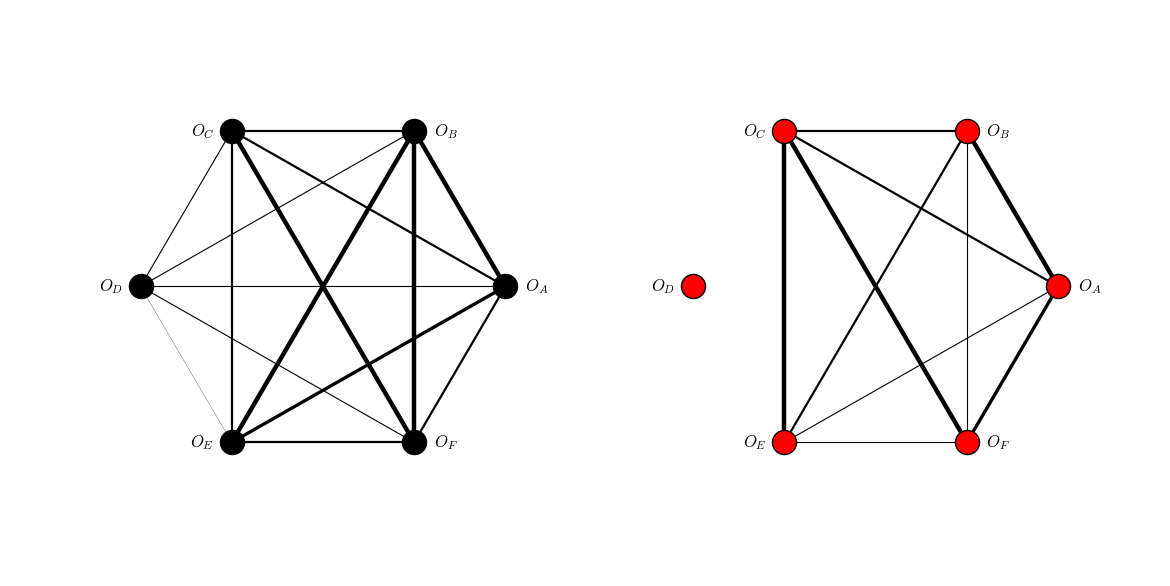
\includegraphics[scale=0.5]{figures/ramping_parameter_example.png}
	\caption{
Stylized portfolio of six obligors (A, B, C, D, E, and F).
The relative strength of the inter-obligor connections $\rho_{ij}$ is illustrated by the line-width.
In the left figure, the interdependency between customer $D$ and the other customers is rather small.
Additional to the individual inter-customer correlation each customer also has an individual obligation (symbolized by the differently coloured circles), indicated as $O_i$, $i \in \{A, B, C, D, E, F \}$.
Both the obligation of the individual customer $O_i$ and the inter-customer correlations $\rho_{ij}$ are required to compute the Concentration Risk as suggested by our measure.
For a particular value of the correlation strength obligor $D$ becomes independent from all other obligors of the portfolio.
	}
	\label{fig:6_pf_ramping}
\end{figure}

 
 
% And the next is a somewhat informal definition
 
\begin{definition}{Portfolio}
A credit portfolio is a tuple $(O, \hat{\rho})$, where $O$ is a set of $n$ exposures from $n$ different obligors and $\hat{\rho}$ an $n \times n$ matrix.
The $\rmat$ matrix represents the interdependency (or correlation) between each obligor $i$, and each element $\rij \in [0,1]$.
\end{definition}

\begin{remark}
Throughout this work, the matrix $\rmat$ is symmetric, so that $\forall i,j \rij = \rho_{ji}$ and the values of $\rho_{ij}$ are positive.
Even though in the real world the dependency between obligors is not necessarily symmetric, e.g. in the case where obligor $i$ is asubsidiary of obligor $j$, the symmetry assumption renders the model more analytically tractable.
\end{remark}





The algorithm is described in~\ref{algo:ramping_parameter}.

\begin{algorithm}
\label{algo:ramping}
\caption{Ramping parameter algorithm~\label{algo:ramping_parameter}}
\State $\ramp \gets 0$

\State $w$ \gets \textrm{order $O_{ij}$}

\State $C$ \gets \{\}

\State $\epsilon\gets \min\{w_{ij}\}$

% 1. We systematically increase the ramping parameter ρ∗ from 0 to 1 with a suffi- ciently small step size.
\For{$\ramp$ \in [0,1]}

	M \gets \text{compute the obligor correlation matrix as shown in eq~\ref{}

	G \gets ({O, {m_{ij}})

	C \gets \text{all connected connected components of graph} G

	R(\ramp) \gets \max_{C_k} \left(  \frac{\sum_{j\in C_k} \textrm{EAD}_j}{\sum_i \textrm{EAD}_i}  \right), where C_k\\

\EndFor
\end{algorithm}

% 2. For each value of ρ∗ we compute the effective (inter) obligor-correlation matrix as shown in Eq. 3.2.
% 3. We compute the number of connected components and the corresponding obli- gation in each component of the graph for every value of ρ∗.4
% 4. To properly account for the Concentration Risk we compute the ratio R(ρ∗) of the maximum of all exposures of all identified connected components Ck and the total exposure of the portfolio
% of the portfolio and j runs over all loans within the connected component Ck.

% In Eq. (3.3) i runs over all loans of the portfolio, i EADi is the total obligation
% Note that R(ρ∗) describes the risk of a portfolio associated with the default of its biggest clump for a given ρ∗. The risk related to a correlated default of the two biggest clumps - which has a very small probability - is not included in equation (3.3). Of course one could account for such scenarios in R(ρ∗) as well by adjusting formula (3.3). As correlated defaults are exponentially suppressed we do not incorporate them in


% section the_ramping_parameter_model (end)

\section{Ramping parameter under random graph model} % (fold)
\label{sec:ramping_parameter_under_random_graph_model}


In this section, we will using properties of the random graph model in order to make predictions about the ramping parameter and the concentration risk.
Contrasting to the original work on the ramping parameter~\cite{Sindel:2009vd}, rather than computing the concentration risk of a particular portfolio, we wish to see the behaviour of the family of portfolios drawn from a given distribution.
In order to do this, certain assumptions about the portfolios must be made.
In particular, we assume:
\begin{itemize}
	\item the portfolios to be large, i.e. we assume that $n \rightarrow \infty$, where $n$ is the number of obligors
	\item the exposure of each individual obligor is $\frac{1}{n}$, i.e. the exposure is uniformly distributed amongst all obligors
	\item the elements of the dependency matrix to be independent from each other
\end{itemize}

\begin{remark}The dependency to large $n$ allows the results for the random graph model to hold exactly.
In practice, however, even large portfolios will be finite and there will be some error.
\end{remark}




\begin{theorem}{Equivalence to random graph model}
\label{thm:equivalence_rgm}
Consider the following probability spaces:
\begin{itemize}
	\item the space of correlation matrices $(\mathcal{C}_m)$
	\item the space of unweighted adjacency matrices $(\mathcal{A}_m)$
	\item the space of random graphs $G_{n,p}$
\end{itemize}
The probabilistic spaces are equivalent.
\end{theorem}
\begin{proof}
\end{proof}

\begin{theorem}{Equivalence to random graph model}
\label{thm:equivalence}
Let $M$ be a square symmetric random matrix with size $n \times n$ whose elements $m_{ij}$ are statistically independent and follow some continuous or discrete distribution $f$.
Let $F$ be the c.d.f. of this distribution.
Let $\tau \in [0,1]$ be a threshold parameter and define $$M_1 = \begin{cases}
1 & \text{if  } m_{ij} \ge \tau\\
0 & otherwise.
\end{cases}$$
Then, the graph defined by the adjacency matrix $M_1$ belongs to $G_{n, 1-\tau}$.
% - Ramping(Random Matrix) = Random Graph?
\end{theorem}
\begin{proof} The random graph model is defined by two conditions:
\begin{enumerate}
	\item every edge exists independently
	\item every edge exists with fixed common probability $p$.
\end{enumerate}
(1) By definition, every element of $m_{ij}$ from $M$ is drawn independently from each other, so condition (1) is met.\\
(2) each of the elements $m_{ij}$ are drawn from the same probability distribution. By the definition of the c.d.f. and $M_1$, with probability $\tau$ their value in $M_1$ will be $0$ (no edge exists) and probability $1-\tau$ the value will be $1$ (edge exists).
\end{proof}
\todo{Discuss with Walter}
\vspace{0.5cm}

Theorem~\vref{thm:equivalence} allows us to apply the results of the random graph model to the study of the ramping parameter, by making some assumptions on the distribution of the portfolio interdependency matrix $\rmat$.
In particular, the original work of~\cite{Sindel:2009vd} assumes $\rhoij$ to be a non-negative correlation value in the interval $[0,1]$, without making any particular assumptions on the distribution of the values.

In practice the matrix $\rmat$ can be generated by multiplying a set of (independent or correlated) risk factors with the dependencies of each obligor to these risk factors.
\todo{example}
Alternatively, it could also be generated either by expert knowledge (in which case one would expect the matrix to be rather sparse), by a pure correlation of stock prices of the obligors, or even by a hybrid approach.

In light of this, no general assumptions can be made over the distribution of the values of $\rmat$ and we will be studying the behaviour of the ramping parameter under the following distributions:
the uniform distribution,
the exponential distribution.


Uniform distribution, means that sampling from the random graph model is the same as generating a random portfolio and applying the ramping parameter.


\subsection{Giant component} % (fold)
\label{sub:giant_component}

As seen in section~\vref{sub:giant_component}, \vref{eq:s_giant_component_lambert} the giant component of the $G_{n,m}$ exists when $c \ge 1$, $c$ being the mean degree of $G$, and has relative size $S$ given by:
\begin{equation}
	S = 1 + \frac{W(-c e^{-c})}{c}
\end{equation}


\subsubsection{Uniform distribution} % (fold)
\label{ssub:uniform_distribution}

By assuming that the $\rij$ are distributed uniformly between $[0,1]$

% subsubsection uniform_distribution (end)

\subsubsection{Truncated exponential distribution} % (fold)
\label{ssub:truncated_exponential_distribution}

By assuming that the $\rij$ are distributed uniformly between $[0,1]$

% subsubsection uniform_distribution (end)



% subsection giant_component (end)

\subsection{Component sizes} % (fold)
\label{sub:component_sizes}

Using the random graph model we know the distribution of the sizes of the connected components.
From the previous chapter, we know that
\begin{equation}
	\pi_s = \frac{1}{s!}\left[  \frac{d^{s-1}}{dh^{s-1}}e^{s c(h-1)}  \right] = \frac{e^{-s c} (s c)^{s-1}}{s!}
\end{equation}


% subsection component_sizes (end)









\begin{figure}[tb]
	\centering
	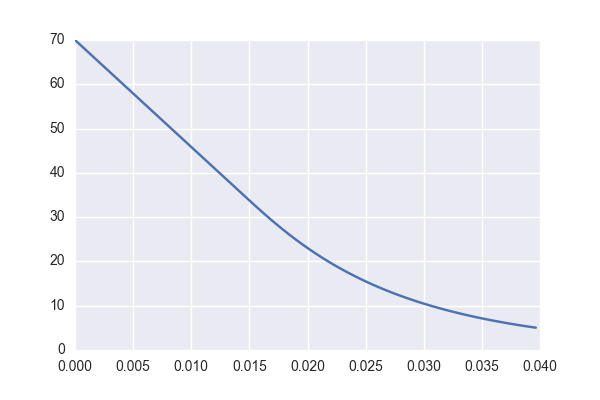
\includegraphics[]{figures/gnp_number_components.png}
	\caption{Number of components as a function of the probability $p$ of the $G(n,p)$ model.}
	\label{fig:figure1}
\end{figure}


\begin{itemize}
	\item The variation of the ramping parameter is equivalent to having random graphs generated with different $p$ probabilities.
\end{itemize}


describe the phase transition


describe the size of the components

% section ramping_parameter_under_random_graph_model (end)

% chapter ramping_parameter_under_the_random_graph_model (end)